\documentclass[11pt]{exam}

\usepackage{amsmath, amssymb, amsthm, multicol}
\usepackage{graphicx}
\usepackage{textcomp}
\usepackage{tikz}

\def\d{\displaystyle}
\def\b{\mathbf}
\def\R{\mathbb{R}}
\def\Z{\mathbb{Z}}
\def\N{\mathbb{N}}
\def\pow{\mathcal{P}}
\def\st{~:~}
\def\bar{\overline}
\def\inv{^{-1}}
\def\imp{\rightarrow}
\def\and{\wedge}

\newcommand{\vtx}[2]{node[fill,circle,inner sep=0pt, minimum size=7pt,label=#1:#2]{}}
\newcommand{\va}[1]{\vtx{above}{#1}}
\newcommand{\vb}[1]{\vtx{below}{#1}}
\newcommand{\vr}[1]{\vtx{right}{#1}}
\newcommand{\vl}[1]{\vtx{left}{#1}}
\renewcommand{\v}{\vtx{above}{}}

%\pointname{pts}
\pointsinmargin
\marginpointname{pts}
\addpoints
\pagestyle{head}
%\printanswers

\firstpageheader{Math 228}{\bf Practice Problems 10: Graph Theory}{Spring 2012}


\begin{document}
\noindent \textbf{Instructions}: The problems below are purely for you to practice.  I will not collect these, but it is still a good idea to write out your solutions in full.  Any of these problems or problems similar are fair game for quizzes and exams.  

\begin{questions}

\question If 10 people each shake hands with each other, how many handshakes took place?  What does this question have to do with graph theory?

\question Among a group of 5 people, is it possible for everyone to be friends with exactly 2 of the people in the group?  What about 3 of the people in the group?

\question You and your friends want to tour the southwest by car.  You will visit the nine states below, with the following rather odd rule: you must cross each border between neighboring states exactly once (so, for example, you must cross the Colorado-Utah border exactly once).  Can you do it?  If so, does it matter where you start your road trip?  What fact about graph theory solves this problem?

\centerline{\includegraphics[height=1in]{images/southwest_map.png}}

\question Which (if any) of the graphs below are the same?  Which are different?  Explain.

\begin{center}
  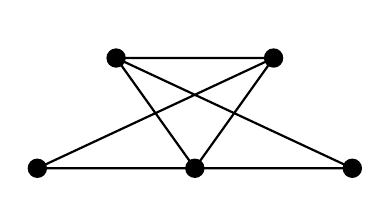
\begin{tikzpicture}[yscale=.7]
    \draw[thick] (-2,0) \v -- (0,0) \v -- (2,0) \v -- (-1,2) \v -- (1,2) \v -- (0,0) -- (-1,2) (1,2) -- (-2,0);
  \end{tikzpicture}
  \hfill
  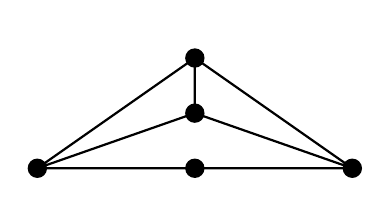
\begin{tikzpicture}[yscale=.7]
    \draw[thick] (-2,0) \v -- (0,0) \v -- (2,0) \v -- (0,1) \v -- (-2,0) -- (0,2) \v -- (2,0) (0,2) -- (0,1);
  \end{tikzpicture}
  \hfill
  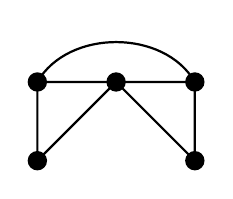
\begin{tikzpicture}[yscale=1]
    \draw[thick] (-1, 0) \v -- (-1,1) \v -- (0,1) \v -- (1,1) \v -- (1,0) \v -- (0,1) -- (-1,0);
    \draw[thick] (-1,1) to [out=60, in=120] (1,1);
  \end{tikzpicture}


\end{center}

\question Which of the graphs in the previous question contain Euler paths or circuits?  Which of the graphs are planar?

\question Is it possible for two {\em different} graphs to have the same number of vertices and the same number of edges?  What if the degrees of the vertices in the two graphs are the same (so both graphs have vertices with degrees 1, 2, 2, 3, and 4, for example)?  Draw two such graphs or explain why not.

\question Which of the following graphs contain an Euler path?  Which contain an Euler circuit?
\begin{parts}
  \part $K_4$
  \part $K_5$.
  \part $K_{5,7}$
  \part $K_{2,7}$
  \part $C_7$
  \part $P_7$
\end{parts}

\question For which $n$ does the graph $K_n$ contain an Euler circuit?  Explain.

\question For which $m$ and $n$ does the graph $K_{m,n}$ contain an Euler path?  An Euler circuit?  Explain.

\question Which of the graphs below are bipartite?  

\begin{center}
  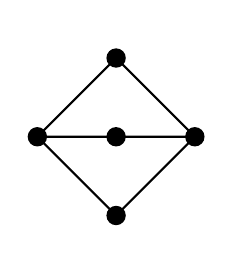
\begin{tikzpicture}
    \draw[thick] (-1,1) \v -- (0,2) \v -- (1,1) \v -- (0,0) \v -- (-1,1) -- (0,1) \v -- (1,1);
  \end{tikzpicture}
  \hfill
  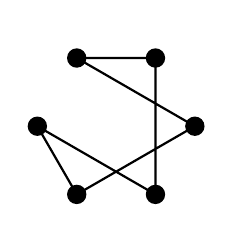
\begin{tikzpicture}
    \draw[thick] (0:1) \v -- (120:1) \v -- (60:1) \v -- (300:1) \v -- (180:1) \v -- (240:1) \v -- cycle;
  \end{tikzpicture}
  \hfill
  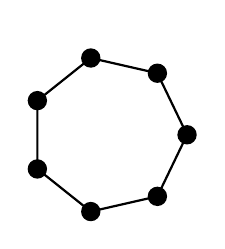
\begin{tikzpicture}
    \draw[thick] (360/7:1) \v -- (2*360/7:1) \v -- (3*360/7:1) \v -- (4*360/7:1) \v -- (5*360/7:1) \v -- (6*360/7:1) \v -- (0:1) \v -- cycle;
  \end{tikzpicture}
  \hfill 
  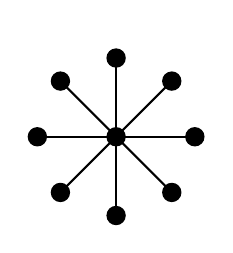
\begin{tikzpicture}
    \draw (0,0) \v;
    \foreach \x in {0,...,7}
    \draw[thick] (0,0) -- (\x*360/8:1) \v;
  \end{tikzpicture}

\end{center}

\question For which $n$ is the graph $C_n$ bipartite?

\question Draw a graph which has an Euler circuit but is not planar.

\question Draw a graph which does not have an Euler path and is also not planar.

\question Is it possible for a planar graph to have 6 vertices, 10 edges and 5 faces?  Explain.

\question If a graph has 10 vertices and 10 edges and contains an Euler circuit, must it be planar?  How many faces would it have?

\question The graph $G$ has 6 vertices with degrees $2, 2, 3, 4, 4, 5$.  How many edges does $G$ have?  Could $G$ be planar?  If so, how many faces would it have.

\question What is the smallest number of colors you need to properly color the vertices of $K_{4,5}$.  That is, find the chromatic number of the graph.

\question Draw a graph with chromatic number 6 (i.e., which requires 6 colors to properly color the vertices).  Could your graph be planar?  Explain.

\question Find the chromatic number of each of the following graphs.

\begin{center}
  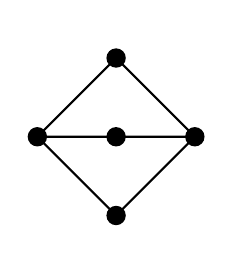
\begin{tikzpicture}
    \draw[thick] (-1,1) \v -- (0,2) \v -- (1,1) \v -- (0,0) \v -- (-1,1) -- (0,1) \v -- (1,1);
  \end{tikzpicture}
  \hfill
  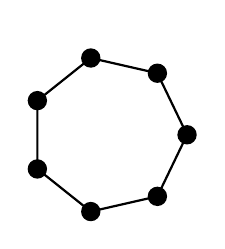
\begin{tikzpicture}
    \draw[thick] (360/7:1) \v -- (2*360/7:1) \v -- (3*360/7:1) \v -- (4*360/7:1) \v -- (5*360/7:1) \v -- (6*360/7:1) \v -- (0:1) \v -- cycle;
  \end{tikzpicture}
  \hfill 
  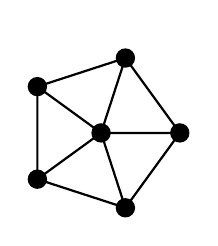
\begin{tikzpicture}
    \draw (0,0) \v;
    \foreach \x in {0,...,4}
    \draw[thick] (0,0) -- (\x*360/5:1) \v -- (\x*360/5+72:1);
  \end{tikzpicture}
  \hfill
  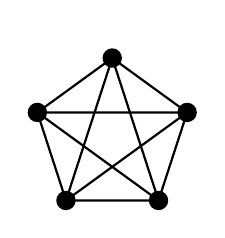
\begin{tikzpicture}
    \foreach \x in {0,...,4}
    \draw[thick] (\x*72+18:1) \v -- (\x*72+90:1) -- (\x*72-54:1);
  \end{tikzpicture}
  \hfill
    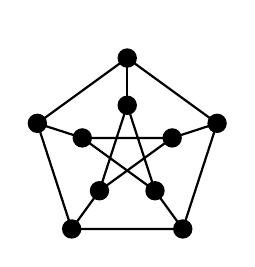
\begin{tikzpicture}[scale=.6]
    \draw[thick] (18:2) -- (90:2) -- (162:2)  -- (234:2) -- (306:2) -- cycle; 
    \draw[thick] (18:1) --  (162:1)  -- (306:1) -- (90:1) -- (234:1) --cycle;
    \foreach \x in {18, 90, 162, 234, 306}
    \draw[thick] (\x:1) \v -- (\x:2) \v;
  \end{tikzpicture}
\end{center}

\question Suppose $G$ is a simple graph with $n$ vertices, each having degree 5. 
\begin{parts}
  \part For which values of $n$ does this make sense?
  \part For which values of $n$ does the graph have an Euler path?
  \part What is the smallest value of $n$ for which the graph might be planar? (tricky)
\end{parts}


\end{questions}


\end{document}


